\documentclass[main.tex]{subfiles}
\begin{document}

\chapter{Evaluation}

In diesem kapitel werden zuvor ausgewählte algorithmen einheitlich verglichen und die resultierenden ergebnisse ausgewertet.

\section{Evaluation Protocol}

To determine the feasibility of performing real-time plane detection, we need to conduct experiments with the selected algorithms.

Another important factor for comparability is the data set, on which the experiments are conducted on.
Because each publication from the presented algorithms uses a different data set for its evaluation, we cannot objectively select an algorithm to be the "best".
Furthermore, to the best of our knowledge, there is no data set, that contains an incrementally growing and unordered point cloud with corresponding ground truth.

Thus, we first evaluate the algorithms on a dataset while excluding the temporal component. We do this by performing plane detection on whole point clouds, rather than
incrementally growing ones. 

We then perform experiments, this time including the temporal component, by performing calculations at each time step and evaluating them individually.

Lastly, through comparison, as well as analysis of those different experiments, a statement will be given as to whether and how well plane detection is
possible in real-time.

For the evaluation of a given dataset, by comparing the test results with the ground truth, we took inspiration from \citeauthor{Araújo_Oliveira_2020} \citedate{Araújo_Oliveira_2020},
especially their \textit{Results} chapter.


\subsection{Metrics}
To quantitatively evaluate an algorithm's performance, we calculate the precision, recall and the f1 score.
First, we regularize the original point cloud to reduce complexity and furthermore to avoid proximity bias, because of the inverse relationship
between distance to sensor and cloud density. This regularization is obtained through voxelization of the point cloud.\\
With this voxel grid, we can now calculate corresponding sets of voxels for each point cloud representing a plane.
In the next step, we compare our planes from the ground truth with the planes obtained from an algorithm to obtain a list of corresponding pairs
of ground truth and found planes.\\
A grund truth plane $p_{gt_i}$ is marked as \textit{detected}, if any plane from the list of found planes achieves a voxel overlap of $\geq 50\%$.
With this list of correspondences, we calculate precision, recall and the f1-score as explained in the following.
For a given ground truth plane $p_{gt_j}$ and a corresponding found plane $p_{a_k}$ we can sort a given voxel $v_i$ into the categories
\textit{True Positive(TP), False Positive(FP) and False Negative(FN)} as follows.
$$v_i \in p_{gt_j} \land v_i \in p_{a_k} \Rightarrow v_{i} \in TP$$
$$v_i \in p_{gt_j} \land v_i \notin p_{a_k} \Rightarrow v_{i} \in FN$$
$$v_i \notin p_{gt_j} \land v_i \in p_{a_k} \Rightarrow v_{i} \in FP$$
% TODO not needed right? $$v_i \notin p_{gt_j} \land v_i \notin p_{a_k} \Rightarrow v_{i} \in TN$$  , True Negative(TN)} 

With those four rules, we can calculate the precision, recall and F1 score like this:
$$Precision = \frac{|TP|}{|TP|+|FP|}$$
$$Recall = \frac{|TP|}{|TP|+|FN|}$$
$$F1 = 2 \cdot\frac{Precision\cdot Recall}{Precision + Recall}$$

Aside from the accuracy, we also need to compare the time each algorithm needs to find its respective set of planes.
For that, we measure the time spent in the plane detection phase, excluding any preprocessing or postprocessing steps.
To measure the detection time, we log the exact times before and after calculations and write the difference to a file.\\

\subsection{Dataset}
To evenly compare algorithms, an appropriate dataset is needed. Through extensive research of current literature, we compiled a list of popular datasets (see Table~\ref{tab:datasets}). 

\begin{table}[]
    \centering
    \begin{tabular}{c|cccc}
        Dataset                                                                                                          & Input Format & Real & Indoor & GT         \\ \hline
        SegComp      \cite{article}                                                                                      & DI  & N    & /      & planes     \\
        S3DIS   \cite{armeni_cvpr16}                                                                                     & UPC    & Y    & Y      & objects    \\
        NYU V2  \cite{10.1007/978-3-642-33715-4_54}                                                                      & DI  & Y    & Y      & classes    \\
        Kinect  \cite{Oehler_efficientmulti-resolution}                                                                  & OPC    & Y    & Y      & planes     \\
        ICL-NUIM       \cite{handa:etal:ICRA2014}                                                                        & DI  & Y    & Y      & trajectory \\
        SYNBEP         \cite{schaefer19icra}                                                                             & OPC    & N    & /      & planes     \\
        ARCO          \cite{Hidalgo-Paniagua_Vega-Rodríguez_Pavón_Ferruz_2015}                                           & OPC    & Y    & Y      & /          \\
        SUN                    \cite{7298655}                                                                            & DI  & Y    & Y      & objects    \\
        Leica          \cite{leica}   & UPC    & Y    & N      & planes     \\
        TUM              \cite{sturm12iros}                                                                              & DI  & Y    & Y      & trajectory
    \end{tabular}
    \caption[Popular Datasets]{Popular Datasets. The \textit{GT}(Ground Truth) column specifies what the ground truth of each dataset represents.}
    \label{tab:datasets}
\end{table}

In Section~\ref{sec:pdaselection}, we select unorganized point clouds (UPC) as input for the selected algorithms. Furthermore, this work focuses on real, indoor environments.
Additionally, a ground truth is necessary for the evaluation.
We select the Stanford Large-Scale Indoor Spaces 3D Dataset(S3DIS)\cite{2017arXiv170201105A} from the list of datasets to evaluate each plane detection algorithm on even grounds.
Since our focus is not on 3D semantic segmentation and the provided ground truth is focused on semantic segmentation rather than planes, we manually select planar regions using CloudCompare\footnote{\href{https://cloudcompare.org/}{https://cloudcompare.org/}}.
S3DIS was recorded in three different buildings and divided into six distinct areas, including 272 different scenes. A detailed statistic of the included scene types can be found in Table~\ref{tab:stanfordStats}.
An individual scene has a complete unstructured point cloud and a list of annotated files representing semantically different objects that can be found therein.

Furthermore, one could argue that an uneven distribution of scene types introduces a particular bias. While it is true that the distribution is quite uneven, the data set nevertheless reflects a realistic distribution of scene types since
it is not realistic that a building contains only lecture halls. On the other hand, it is appropriate to assume that an office complex contains a substantial amount of hallways needed to connect all these offices.

\begin{table}[H]
    \centering
    \begin{tabular}{c|c|c|c|c|c|c|c}
        \hline
        Scene Categories & Area\_1 & Area\_2 & Area\_3 & Area\_4 & Area\_5 & Area\_6 & TOTAL \\ \hline
        office           & 31      & 14      & 10      & 22      & 42      & 37      & 156   \\ \hline
        conference room  & 2       & 1       & 1       & 3       & 3       & 1       & 11    \\ \hline
        auditorium       & -       & 2       & -       & -       & -       & -       & 2     \\ \hline
        lobby            & -       & -       & -       & 2       & 1       & -       & 3     \\ \hline
        lounge           & -       & -       & 2       & -       & -       & 1       & 3     \\ \hline
        hallway          & 8       & 12      & 6       & 14      & 15      & 6       & 61    \\ \hline
        copy room        & 1       & -       & -       & -       & -       & 1       & 2     \\ \hline
        pantry           & 1       & -       & -       & -       & 1       & 1       & 3     \\ \hline
        open space       & -       & -       & -       & -       & -       & 1       & 1     \\ \hline
        storage          & -       & 9       & 2       & 4       & 4       & -       & 19    \\ \hline
        WC               & 1       & 2       & 2       & 4       & 2       & -       & 11    \\ \hline
        TOTAL            & 45      & 39      & 24      & 49      & 55      & 53      & 272   \\
    \end{tabular}
    \caption{S3DIS Disjoint Space Statistics}
    \label{tab:stanfordStats}
\end{table}

\subsection{Real-Life Test}
We record an incrementally growing data set in the Faculty of Computer Science at Otto-von-Guericke University Magdeburg.
To perform a thorough comparison between the static and the dynamic experiment, we record a scene for each of the following scene types of S3DIS:
\begin{itemize}
    \item office
    \item conference room
    \item auditorium
    \item hallway
\end{itemize}

\textcolor{red}{why only them right}

The recorded point clouds can be seen in Figure~\ref{fig:fin}.


Running \textit{realsense-ros} and holding our cameras, we walk through different parts of the building, scanning to the best of our ability.
We save each incremental map update to a file for later usage.

\begin{figure}[H]
    \begin{subfigure}{0.5\textwidth}
        \centering
        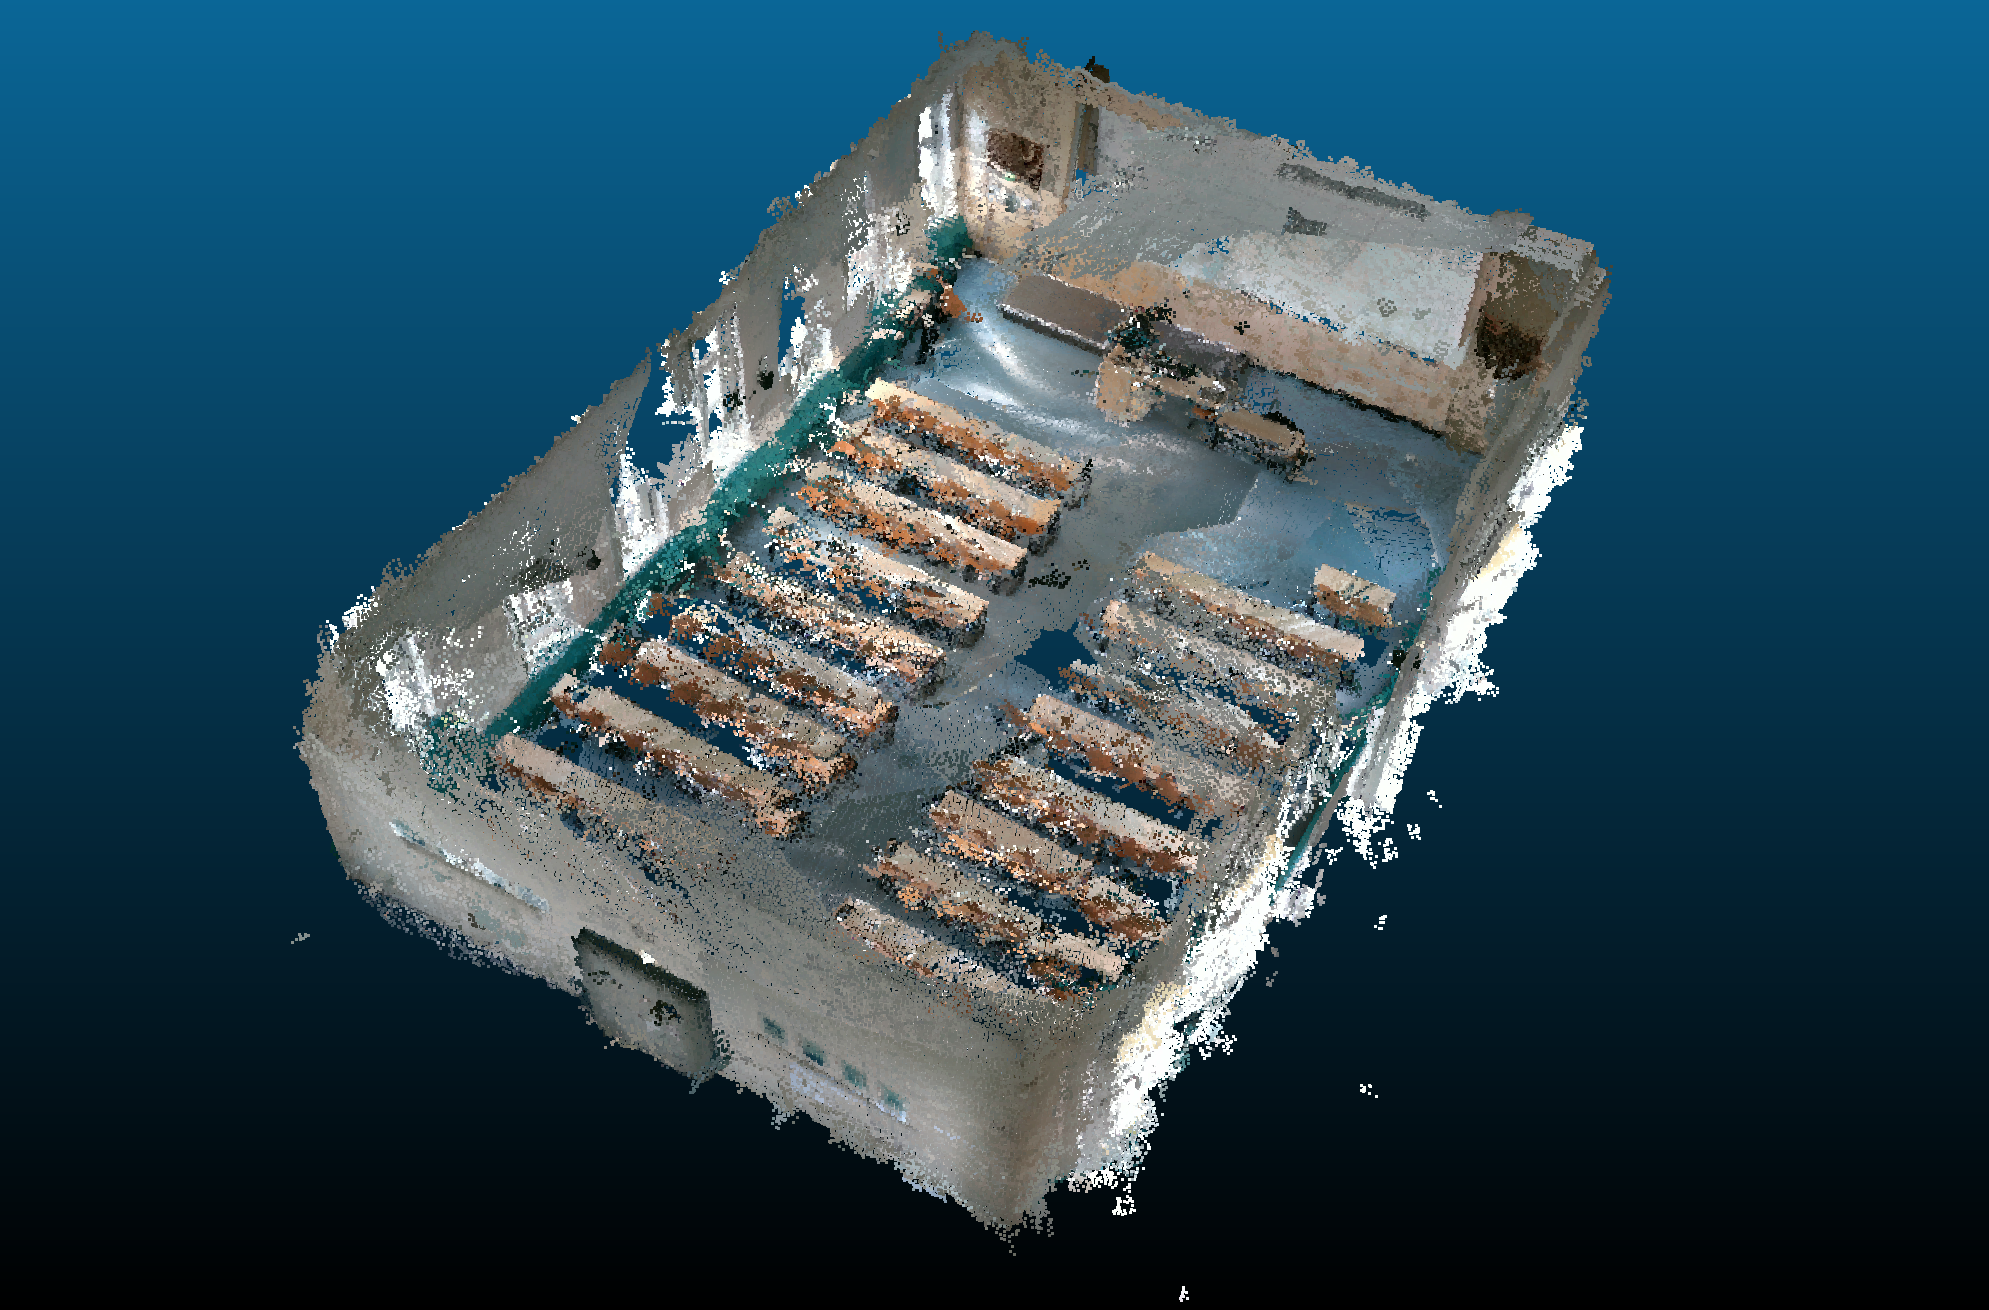
\includegraphics[width=.9\linewidth]{images/307.png}
        \caption[Dynamic Dataset - auditorium]{}
        \label{fig:fin307}
    \end{subfigure}
    \begin{subfigure}{0.5\textwidth}
        \centering
        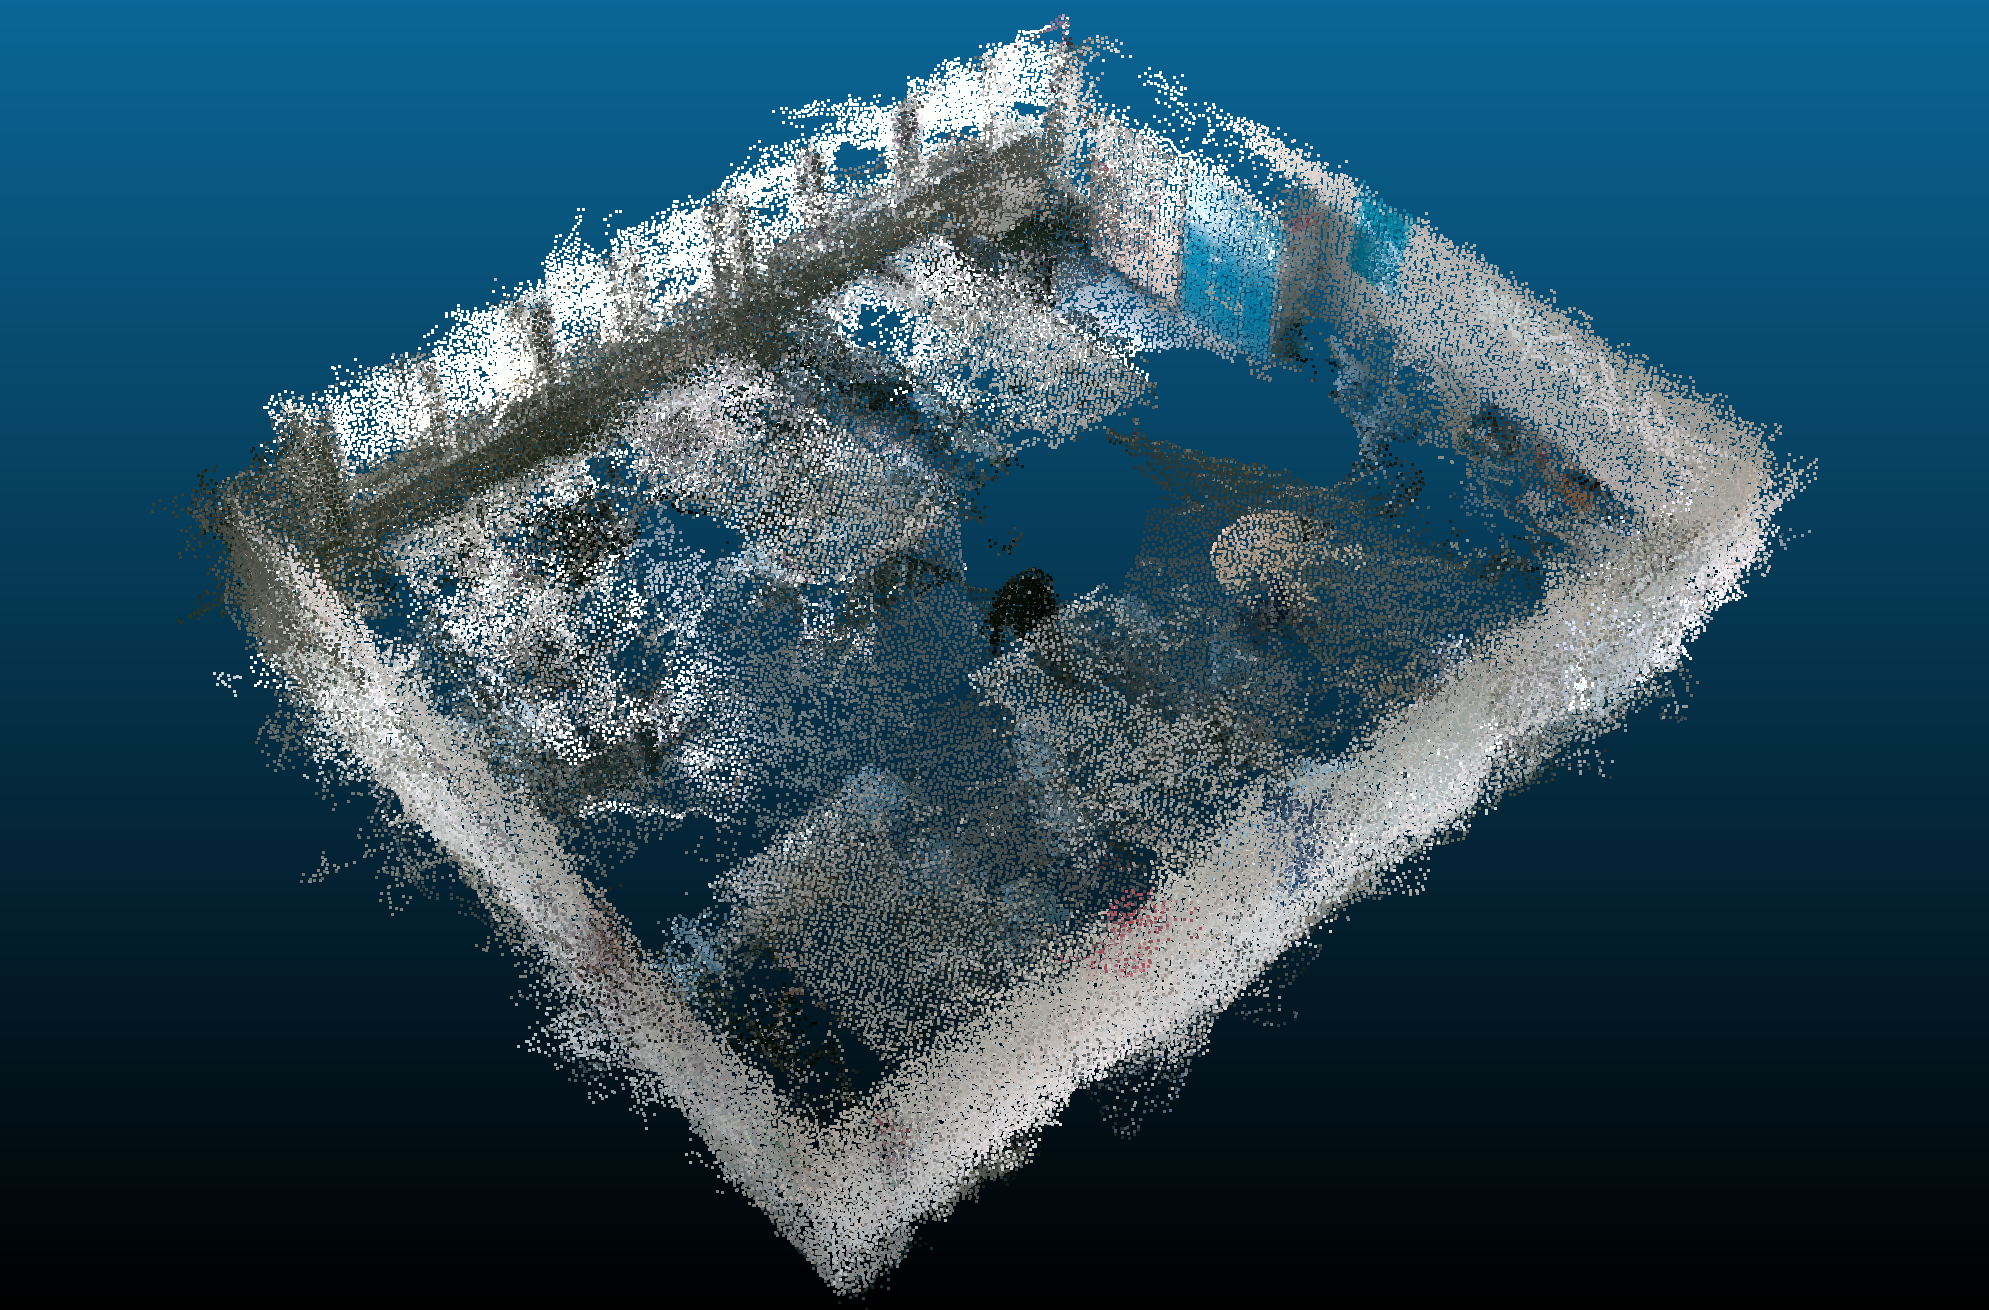
\includegraphics[width=.9\linewidth]{images/333.png}
        \caption[Dynamic Dataset - conference room]{}
        \label{fig:fin333}
    \end{subfigure}
    \begin{subfigure}{0.5\textwidth}
        \centering
        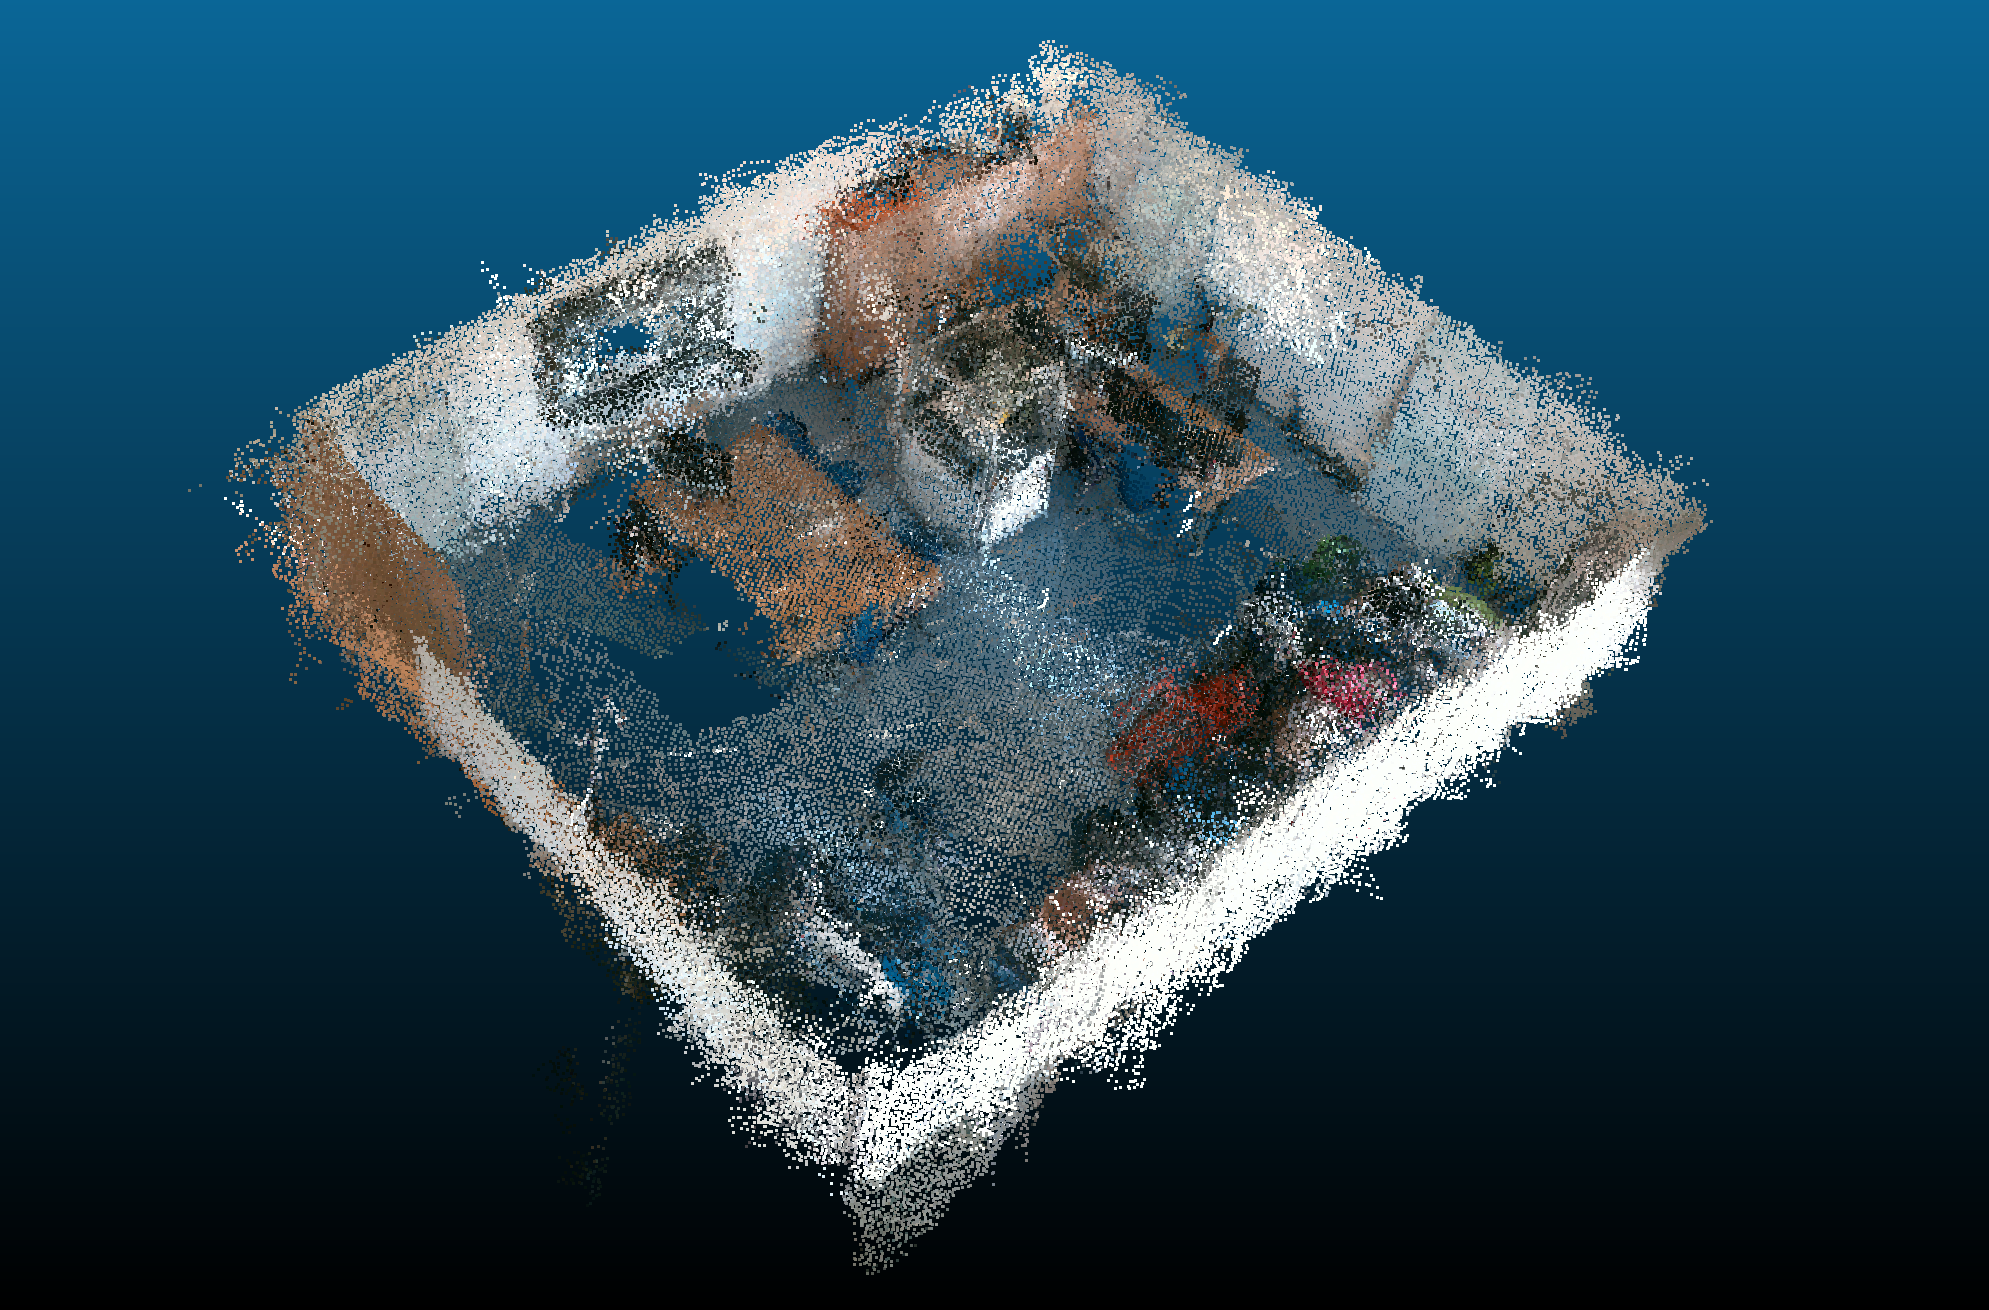
\includegraphics[width=0.9\linewidth]{images/425.png}
        \caption[Dynamic Dataset office]{}
        \label{fig:fin425}
    \end{subfigure}
    \begin{subfigure}{0.5\textwidth}
        \centering
        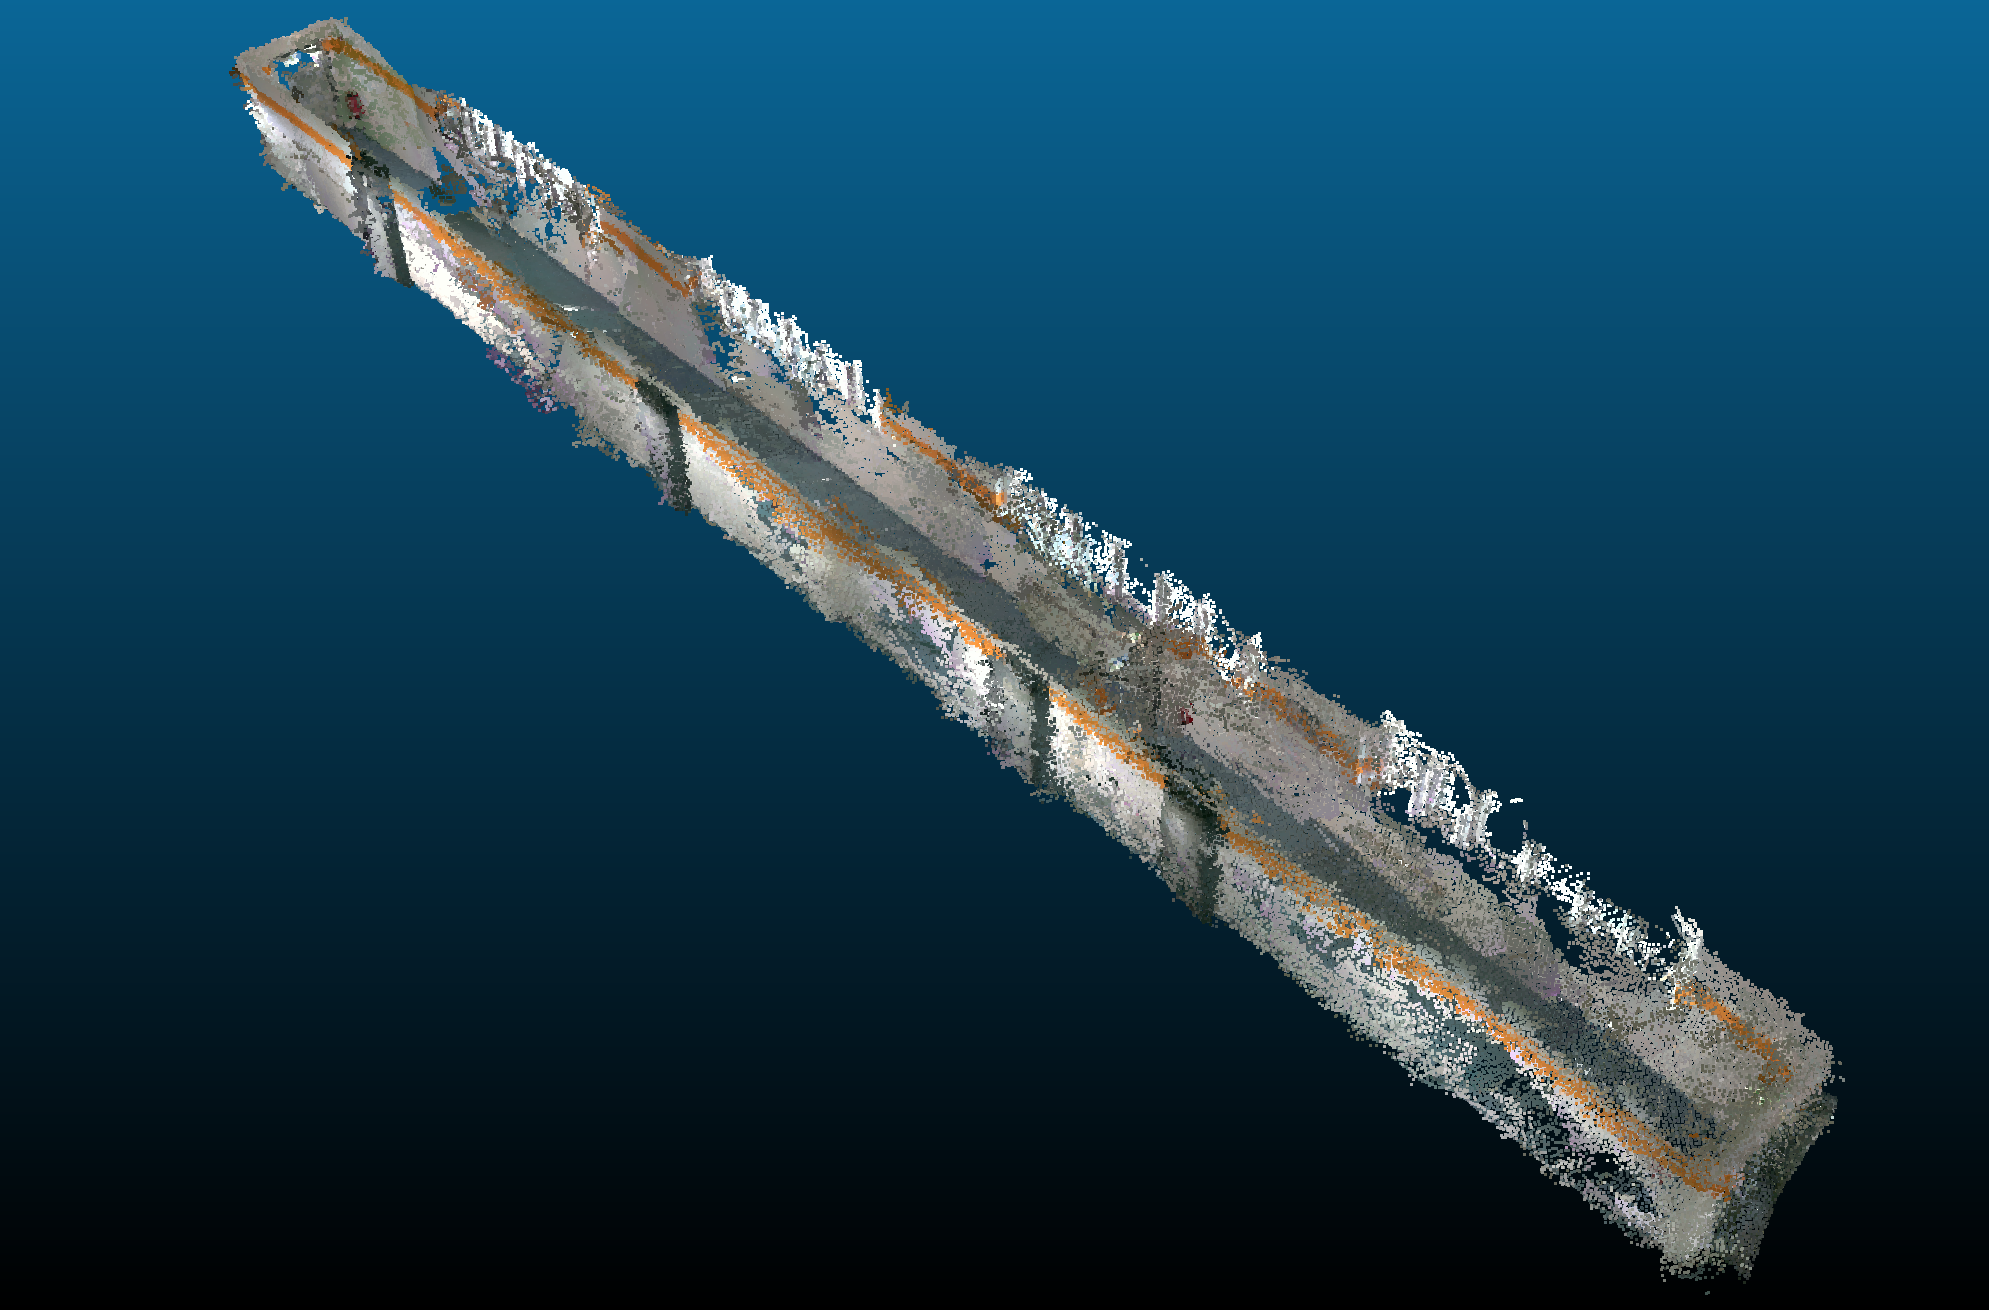
\includegraphics[width=0.9\linewidth]{images/hallway.png}
        \caption[Dynamic Dataset office]{}
        \label{fig:finhw}
    \end{subfigure}
    \caption[Dynamic Datasets]{The recordings for each scene type: (a)auditorium, (b) conference room, (c) office and (d) hallway.}
    \label{fig:fin}
\end{figure}


We create a set of ground truth planes $gt_{end}$ for only the most recent update of each scene, e.g., for the entire recording.
The datasets for
To prepare for the evaluation of a map $m_t$ at a given time $t$, we crop all planes in $gt_{end}$ by removing all points that are not present in $m_t$, as shown in
Figure~\ref{fig:dynGT}.
We speed up this expensive process by employing a KD-Tree neighbor search with a small search radius since we only need to know whether a certain point is present or not.
Furthermore, we remove planes from the ground truth if the number of included points falls short of a threshold.

\begin{figure}[H]
    \centering
    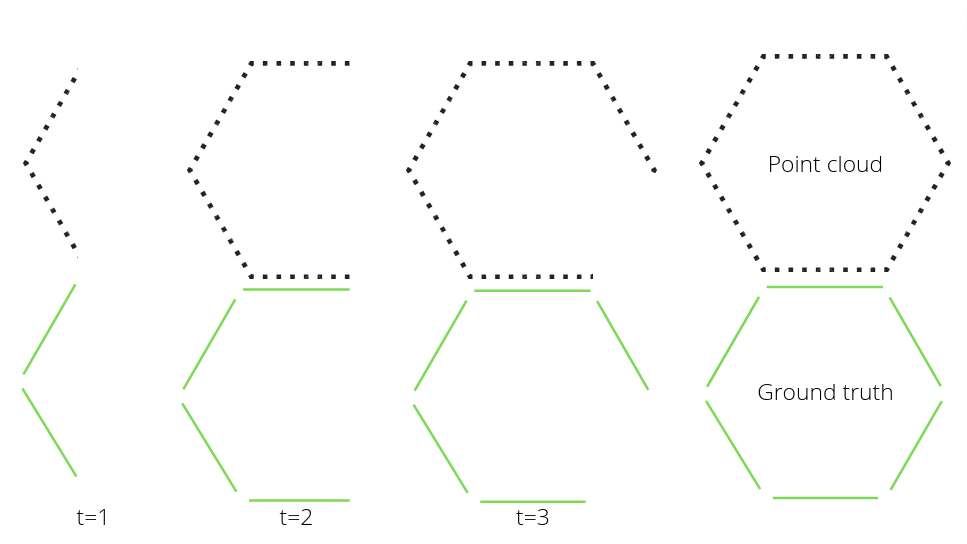
\includegraphics[width=15 cm]{images/dynamic_eval.png}
    \caption[Dynamic Ground Truth Generation]{Dynamic ground truth generation. All planes that are included in \textit{Ground Truth} are cropped depending on
        the available point cloud at each time \textit{t} }
    \label{fig:dynGT}
\end{figure}

\section{Results}
This section deals with the results of the experiments. The individual results of both experiments are presented and analized.

\subsection{Results S3DIS Experiments}

\begin{table}[H]
    \centering
    \begin{tabular}{c|cccc}
              & Precision & Recall & F1   & Time(s) \\ \hline
        RSPD  & 0.85      & 0.89   & 0.86 & 0.90    \\
        OPS   & 0.87      & 0.70   & 0.77 & 16.75   \\
        3DKHT & 0.75      & 0.43   & 0.53 & 0.91    \\
        OBRG  & 0.77      & 0.69   & 0.72 & 44.66
    \end{tabular}
    \caption[Overall S3DIS Results]{Average results of each algorithm over the S3DIS dataset.}
    \label{tab:algo-acc}
\end{table}

Every algorithm performs calculations on every scene included in S3DIS.
The results of each algorithm on an individual scene type are reported in Figure~\ref{fig:stanfordaccuracy} and Figure~\ref{fig:violintime}. As shown in Table~\ref{tab:algo-acc},
RSPD produces the overall best results with an average of 85\% precision, 89\% recall and an F1-score of 86\%, as well as an average of 0.9 seconds of calculation time.
The only other algorithm that achieves similar calculation times is 3D-KHT, which takes 0.91 seconds on average. Considering our definition of \textit{real-time} in Section~\ref{sec:realtime},
RSPD and 3D-KHT are able to perform plane detecion in real-time. Still, 3D-KHT produces the worst overall accuracy results with an average precision of 75\%, recall of 43\%, and an F1-score of 53\%.

With an average of about 17 seconds(OPS) and about 44 seconds(OBRG), both algorithms do not achieve real-time plane detection (see Table~\ref{tab:algo-acc}).


\begin{figure}[]
    \centering
    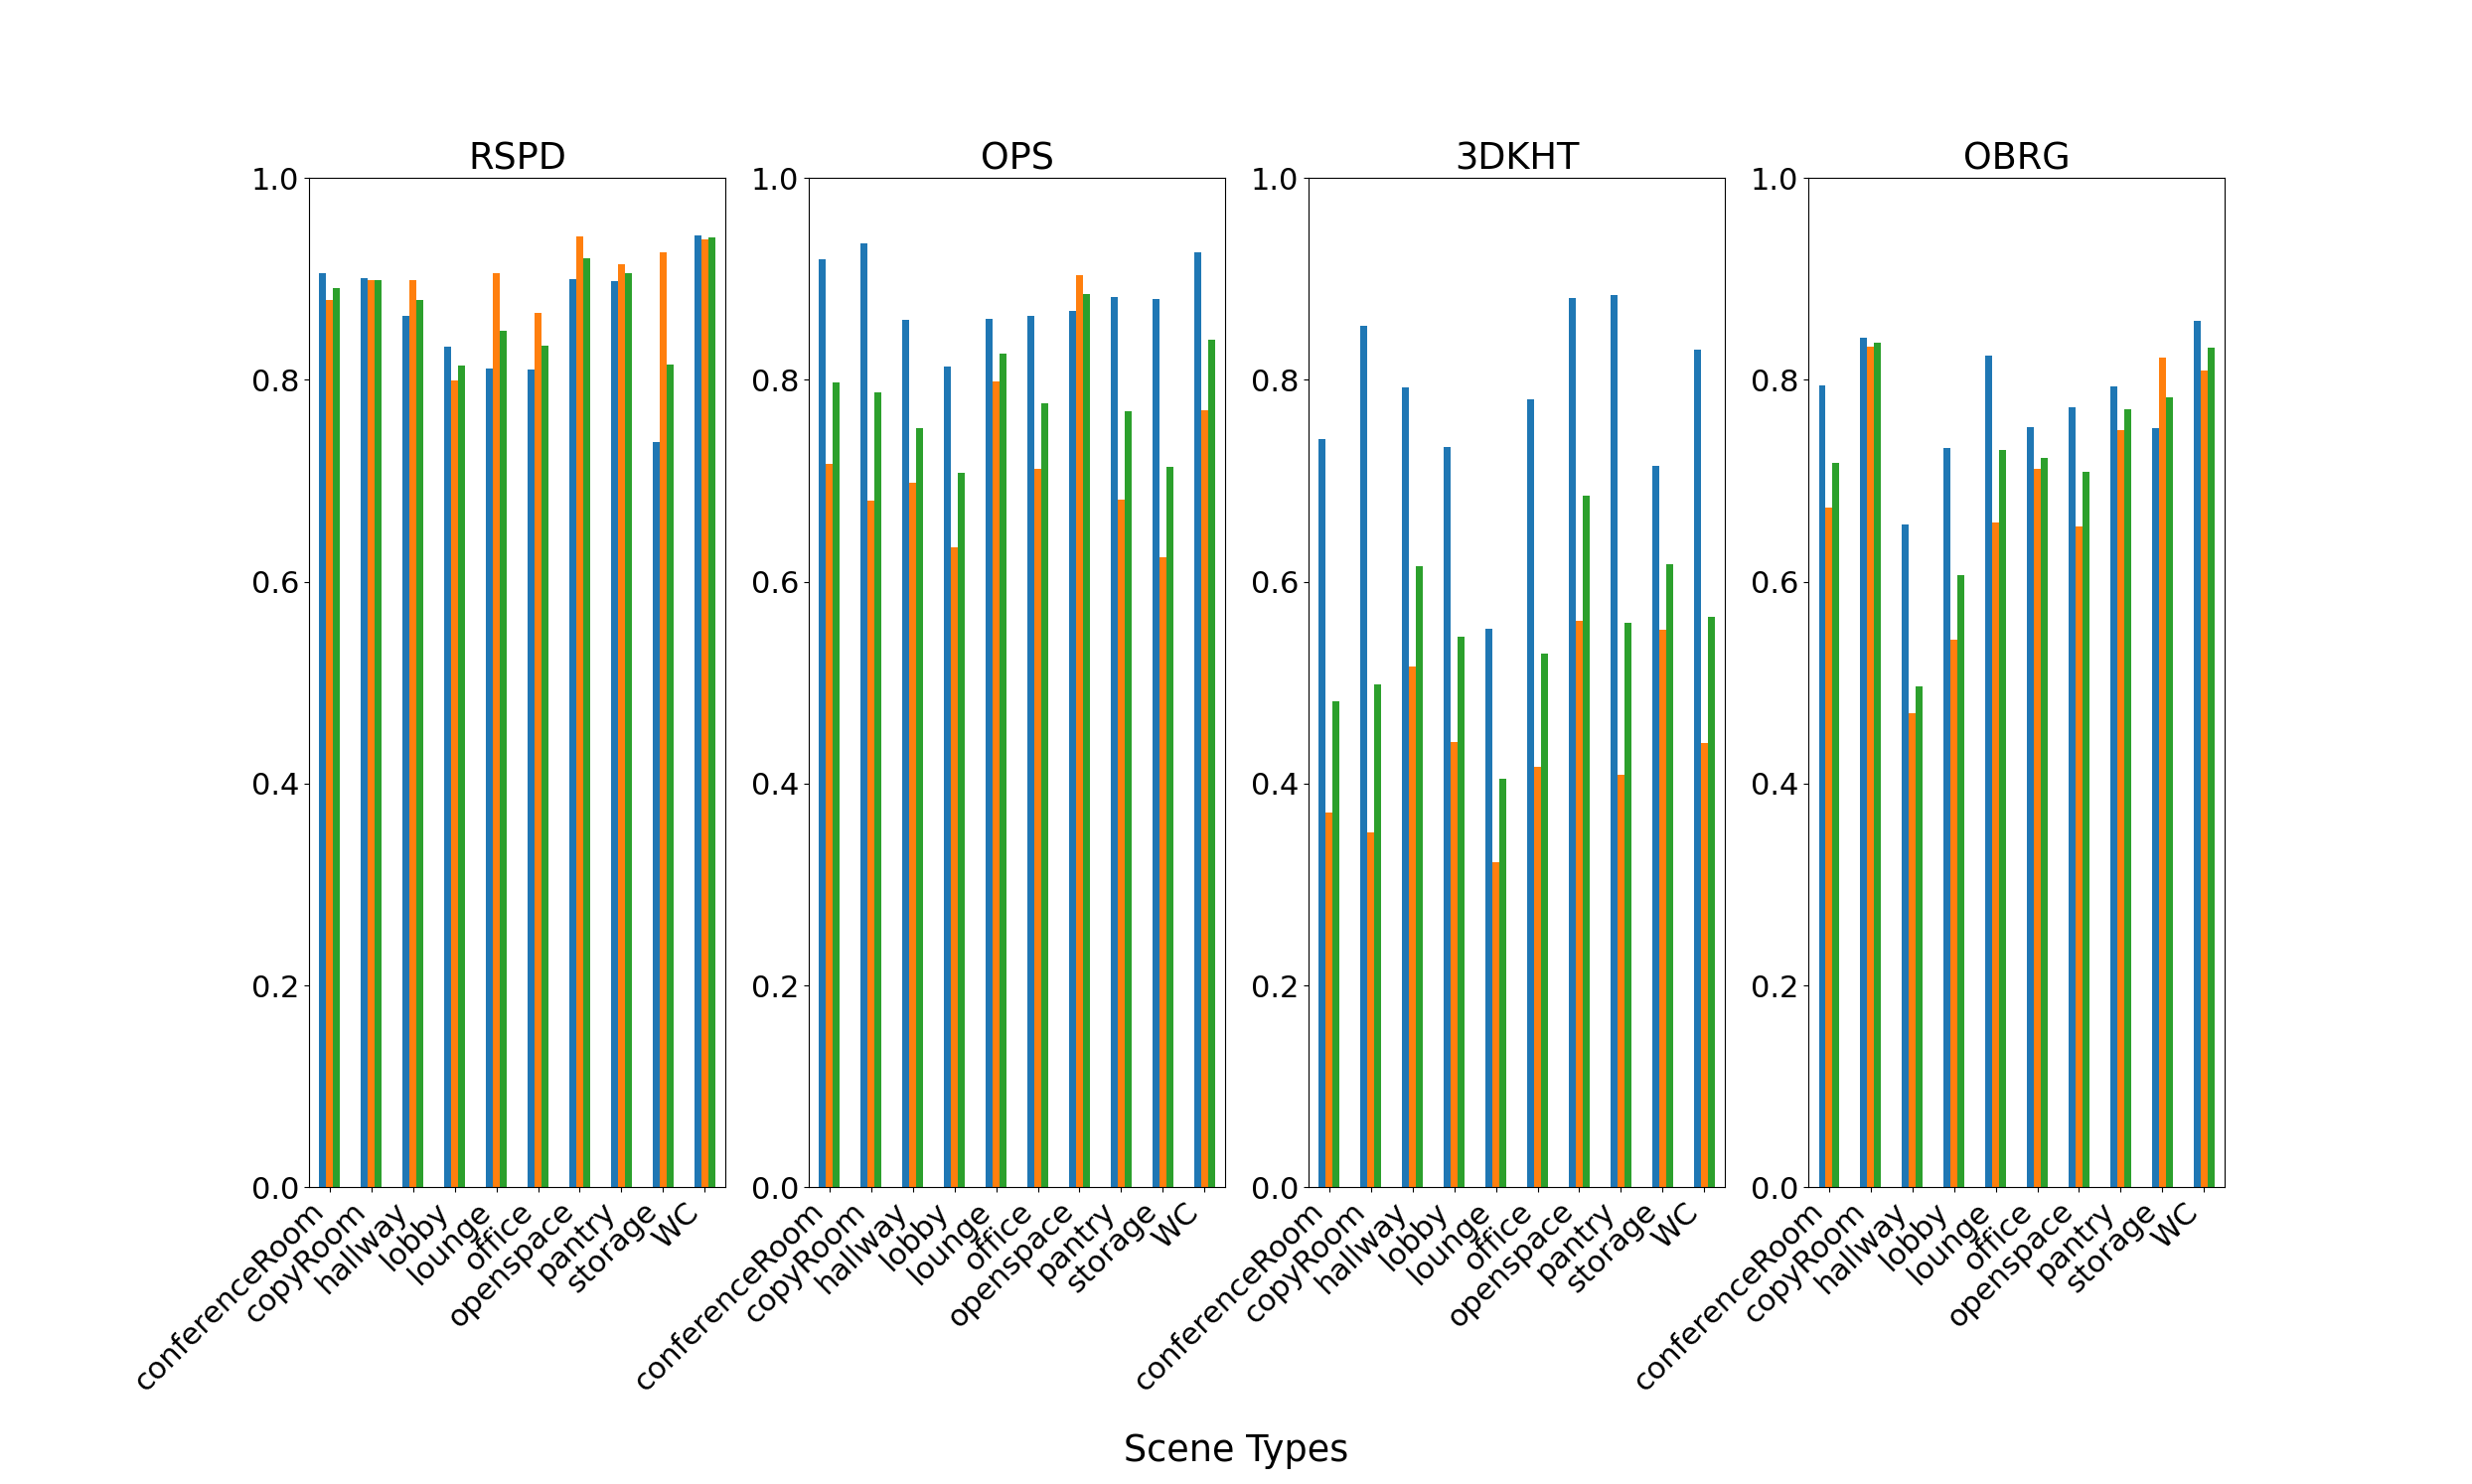
\includegraphics[width=15 cm]{images/accuracy_total.png}
    \caption[Accuracy Results S3DIS]{Average Accuracy for each scene type. The Precision
        is colored blue, recall is orange and the F1-score is green.}
    \label{fig:stanfordaccuracy}
\end{figure}

\begin{figure}[]
    \centering
    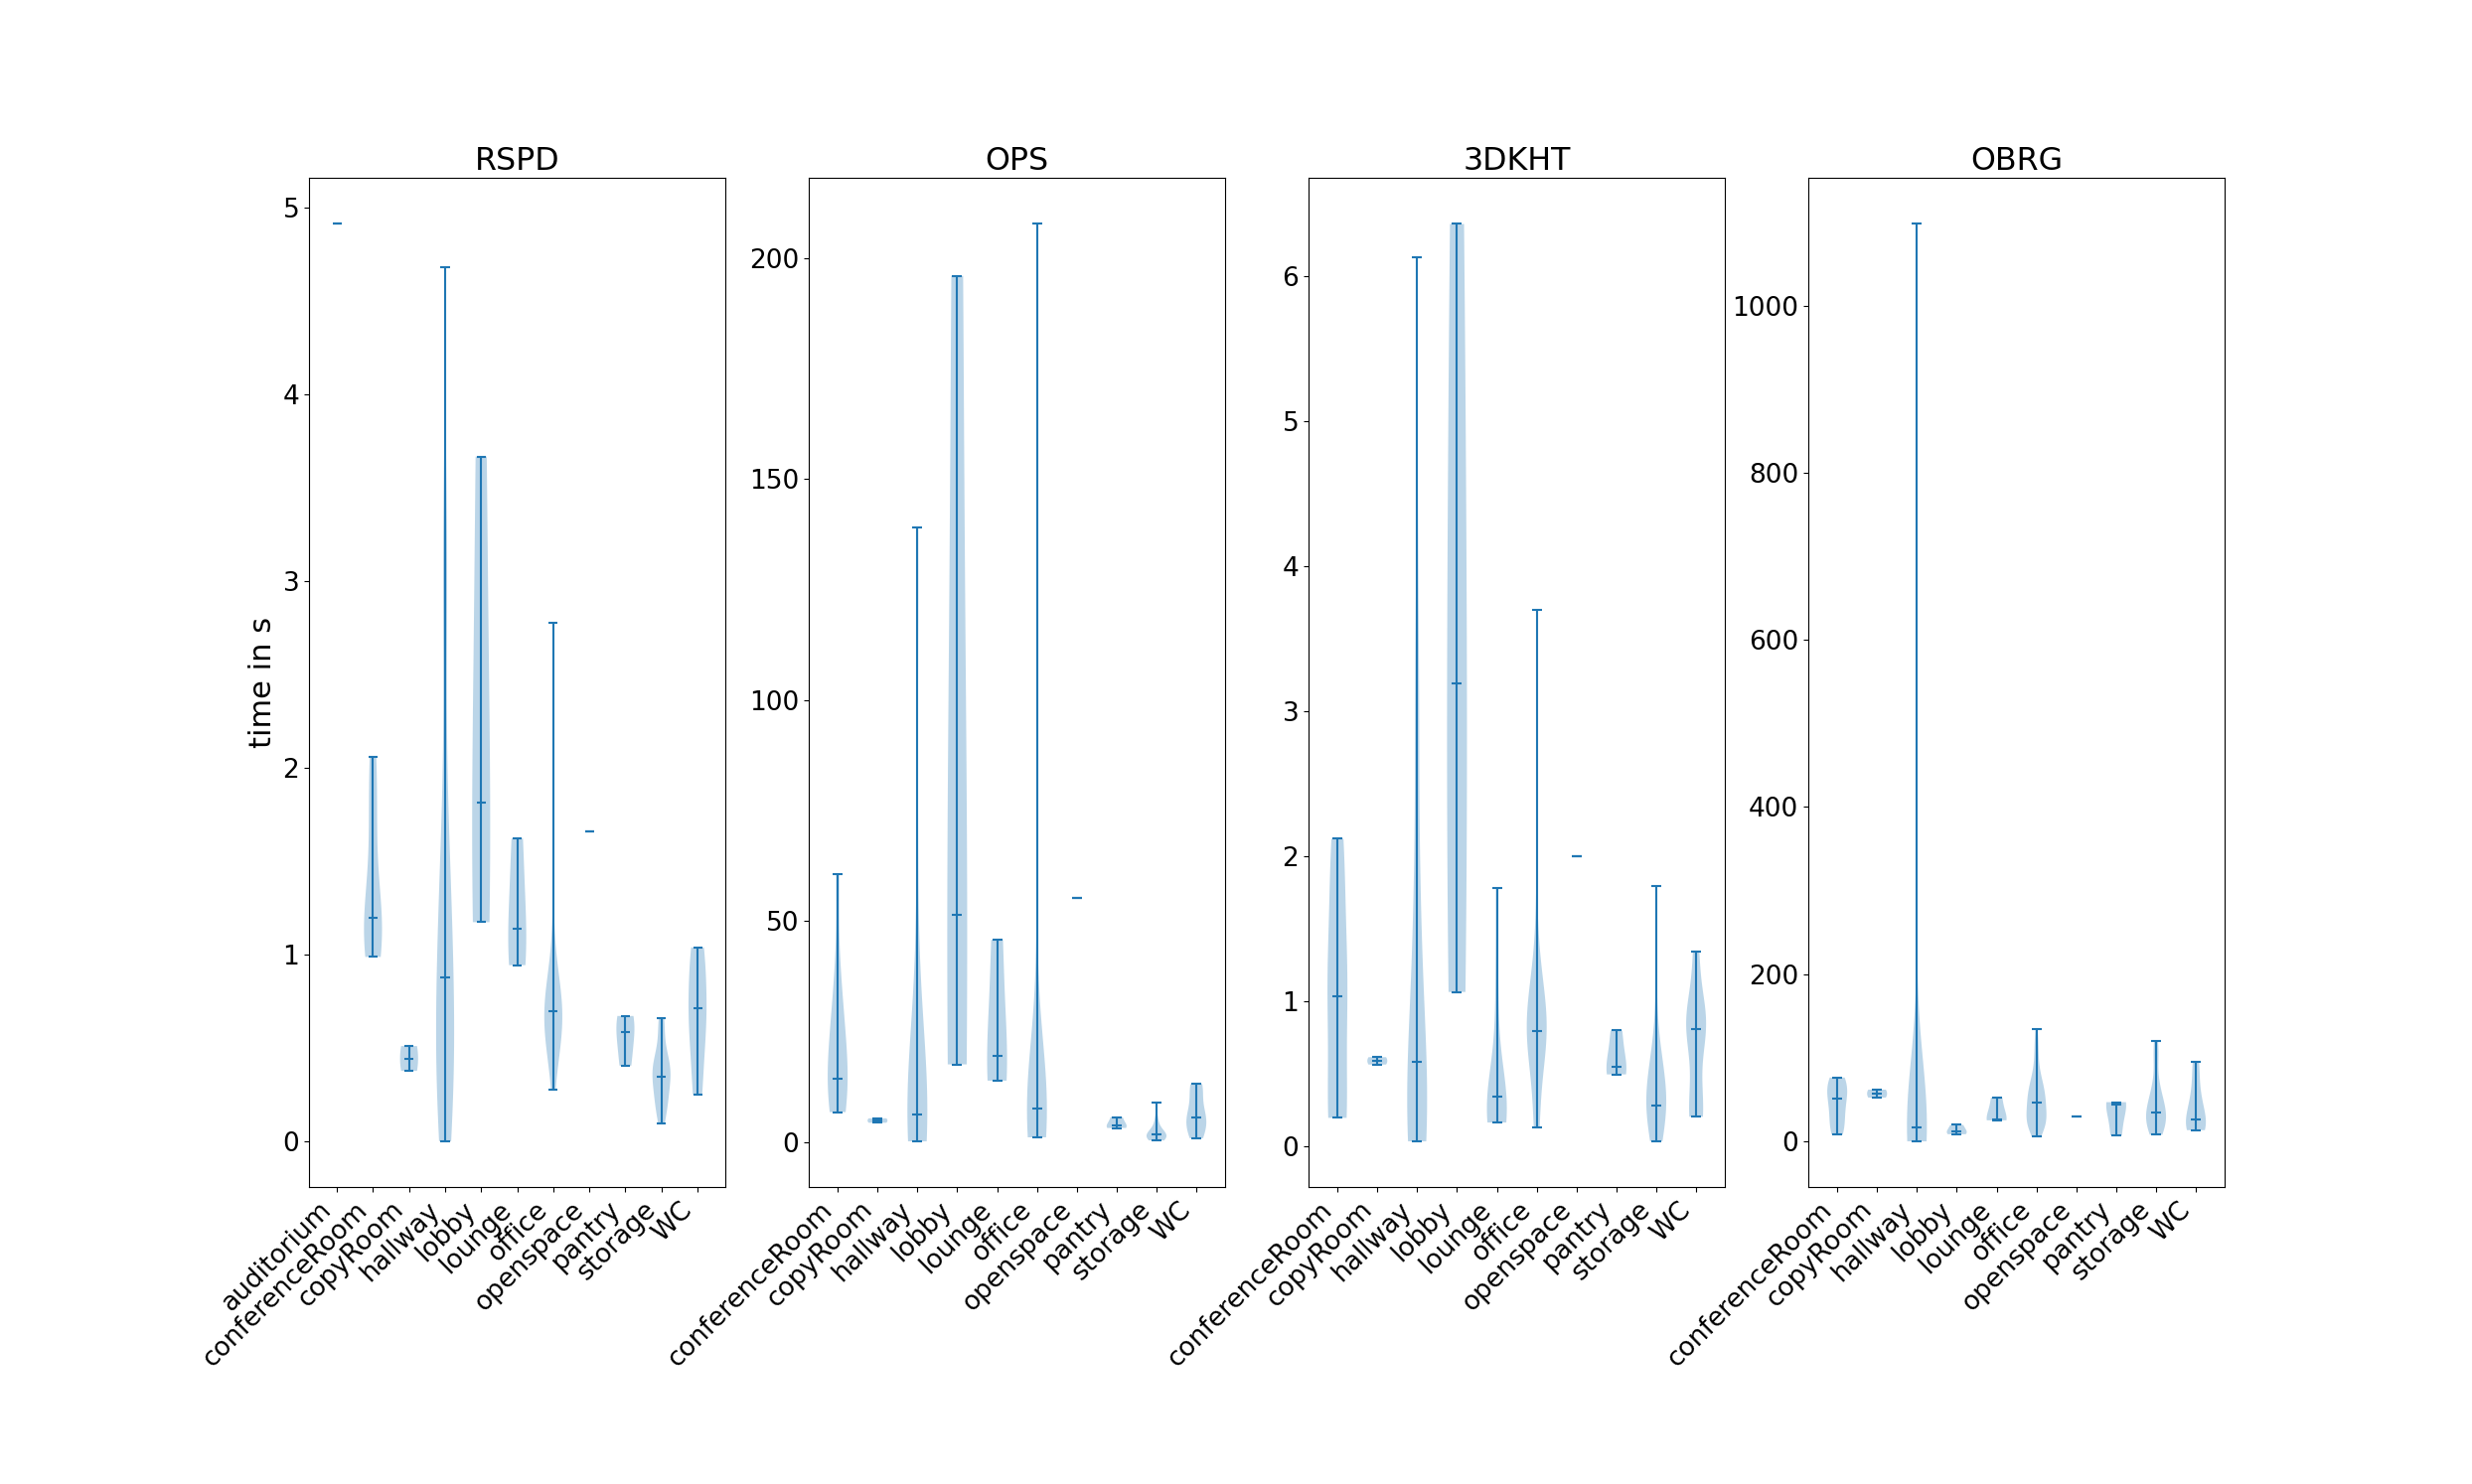
\includegraphics[width=15 cm]{images/times_violin.png}
    \caption[Time Results S3DIS]{Average Time per scene type. Note, that the plots
        do not share the same y-axis.}
    \label{fig:violintime}
\end{figure}

\subsection{Results Real-Life Experiments}
\textit{So far:}

\begin{figure}[]
    \centering
    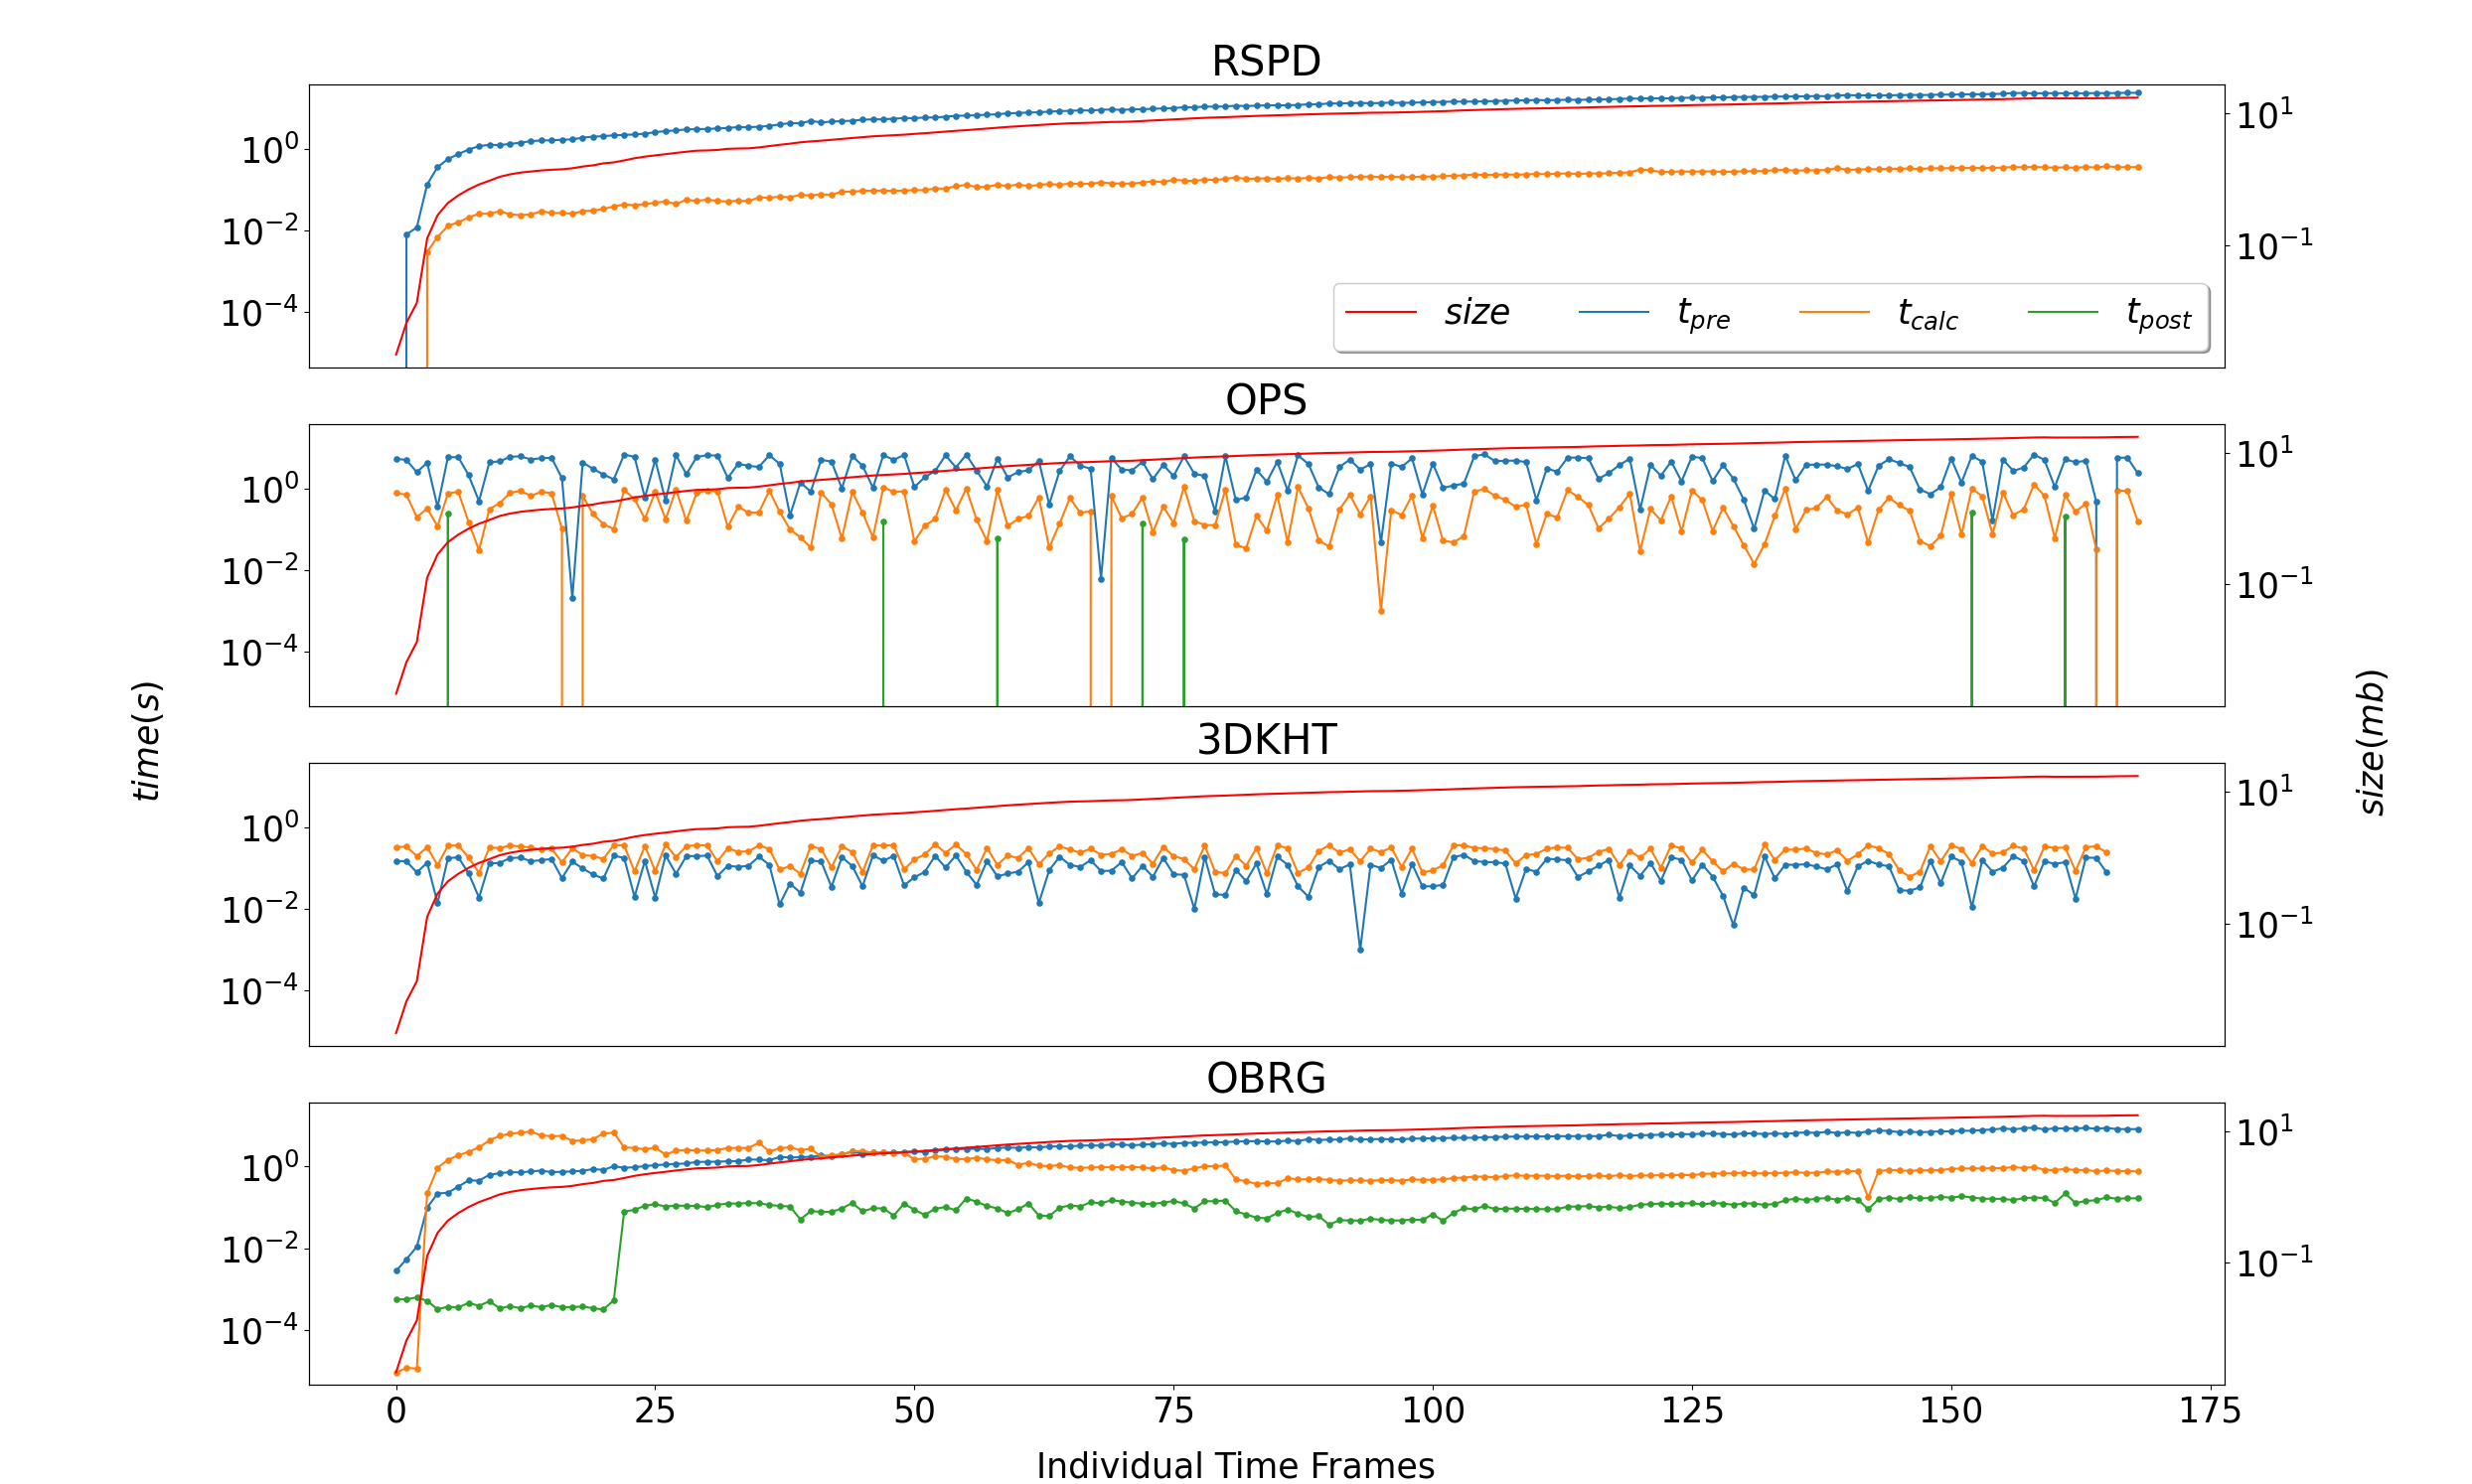
\includegraphics[width=\textwidth]{images/dyn_time-hallway.png}
    \caption[Time Results Hallway]{Calculation times(blue) of the hallway scene and cloud size(red) of each time step.}
    \label{fig:dynhallway}
\end{figure}

The calculation times of all algorithms except OBRG seem to be proportional to the size of the point cloud.
% TODO similar figure for S3DIS
The quality of plane detection, however, decraeses dramatically in comparison to the Stanford Datasets. RSPD is the only dataset that
is able to detect planes. %(see Figure~\ref{fig:}). 


\subsection*{Summary Experiments}
This section combines the preceding results of both experiments.
RSPD is the only algorithm that produces comparable results to the Stanford experiment in the dynamic experiment.
The remaining algorithms cannot reliably detect planes in an incrementally growing environment inheriting varying degrees of noise.

The reason for RSPD's dominance is likely caused by the inherent robustness against noise, as described in Section~

Die ergebnisse der beiden experimente unterscheiden sich in folgendem punkt. Dazu sei gesagt, dass die experimente folgende übereinstimmungen haben.
Das lässt sich so erklären. Alternative gründe davon könnten diese hier sein.

Ich denke RSPD ragt heraus, da hier besonders auf noise resistenz geachtet wurde. % TODO verweis auf diverse noise tests im BG


\end{document}